\lab{Algorithms}{Matrix Operations and Algorithmic Complexity}{Matrices and Complexity}
\objective{This lesson explains basic matrix operations in MATLAB.}

Matrices form the core data structure in MATLAB. As such we investigate several methods of creating and modifying matrices.

To begin we work with vectors. We demonstrate a variety of methods to create vectors. You should follow these demonstrations on your own computer and experiment as you go. Create a vector using square brackets as follows:

\begin{lstlisting}[style=matlab]
>> b = [1 2 3]
b =
     1     2     3  
\end{lstlisting}

We make a column vector by placing semi-colons between the entries.

\begin{lstlisting}[style=matlab]
>> b = [1;2;3]
b =
     1
     2
     3  
\end{lstlisting}

We combine vectors together by placing two or more of equal dimension inside square brackets. The technical term for this is concatenation.

\begin{lstlisting}[style=matlab]
>> c = [4;5;6]
c =
     4
     5
     6
>> d = [b;c]
d =
     1
     2
     3
     4
     5
     6  
\end{lstlisting}

There are several built-in methods to automate vector creation. For example, we can build a vector of consecutive values using the colon operator, a starting value, and an ending value:

\begin{lstlisting}[style=matlab]
>> 1:5
ans =
     1     2     3     4     5
\end{lstlisting}

This syntax also allows us to specify step size:

\begin{lstlisting}[style=matlab]
>> 1:.5:3
ans =
    1.0000    1.5000    2.0000    2.5000    3.0000
\end{lstlisting}

We can similarly use negative step sizes:

\begin{lstlisting}[style=matlab]
>> 3:-.5:1
ans =
    3.0000    2.5000    2.0000    1.5000    1.0000
\end{lstlisting}

A related function is called \li{linspace}. It allows us to specify two endpoints and the number of equidistant values we want between the two.

\begin{lstlisting}[style=matlab]
>> linspace(1,2,5)
ans =
    1.0000    1.2500    1.5000    1.7500    2.0000
\end{lstlisting}

The \li{plot} function uses two vectors to create a graph, the first vector representing $x$-values and the second representing the corresponding $y$-values.  As an example we plot a line of slope two using the following commands (See Figure \ref{fig:graph}):

\begin{lstlisting}[style=matlab]
>> x = linspace(-2,2,20);
>> plot(x,2*x)
\end{lstlisting}

\begin{figure}
\vspace{-100pt}
\begin{center}
	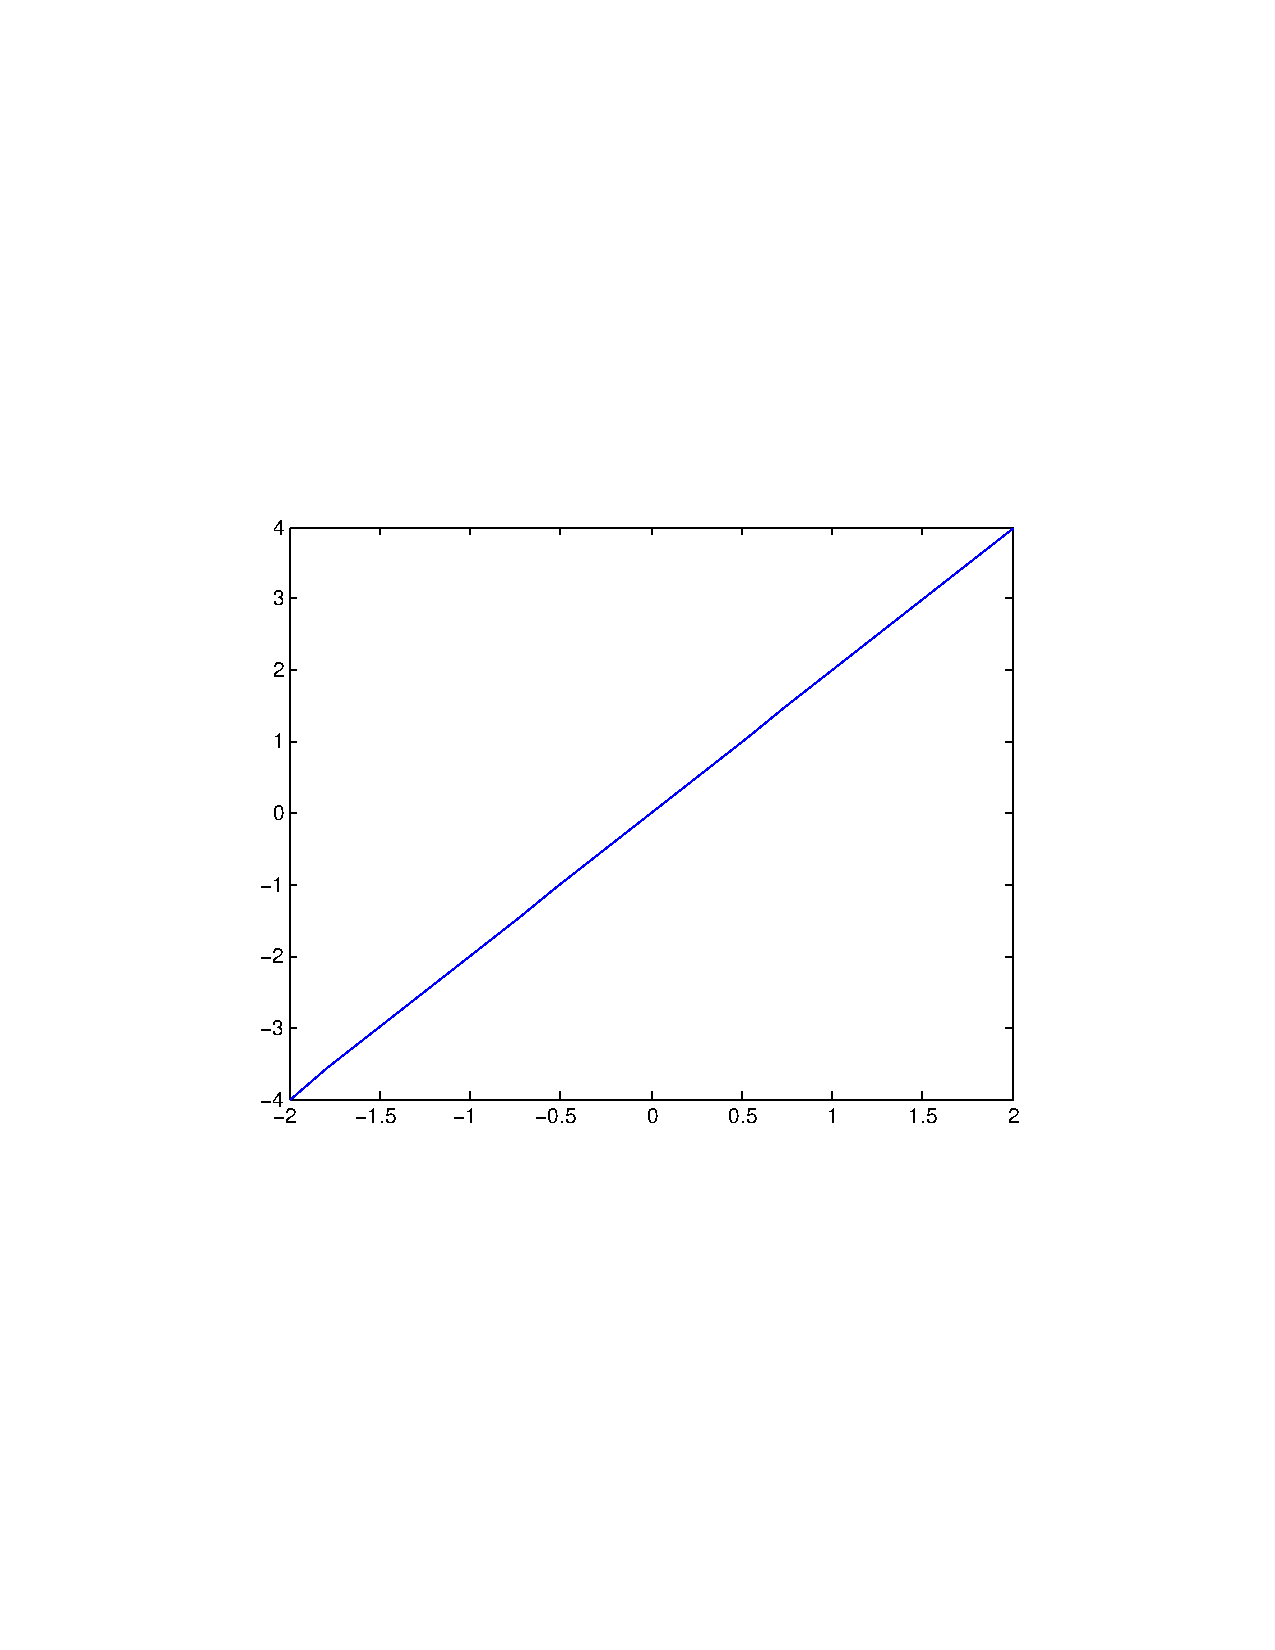
\includegraphics[scale=.5]{./FiguresMAT/graph}
\end{center}
\vspace{-100pt}
\caption{A simple graph}
\label{fig:graph}
\end{figure}

By typing \li{help plot} into the command line we can find the exact syntax and options for the \li{plot} function. For example we can type \li{plot(x,2*x,'r*')} to plot red star data points instead of a line.

\begin{problem}
Plot a line with slope three with black diamond data points. Plot for the domain $x \in [-5,5]$. 
\end{problem}

Creating matrices in MATLAB is done by concatenating vectors in the correct manner. For example:

\begin{lstlisting}[style=matlab]
>> [[1 2 3];[4 5 6];[7 8 9]]
ans =
     1     2     3
     4     5     6
     7     8     9
\end{lstlisting}

\begin{problem}
Create a matrix showing the times table from 1 to 6. Do not enter each number manually. Instead, create a variable \li{x = 1:6} and let the rows of the matrix be multiples of $x$.
\end{problem}

Another technique for creating matrices is using outer products. An outer product is the method of multiplying two vectors to get a matrix. For example, if we want to make a matrix that is two repeated rows of the vector 1:5 we can do the following:

\begin{lstlisting}[style=matlab]
>> [1;1]*(1:5)
ans =
     1     2     3     4     5
     1     2     3     4     5
\end{lstlisting}

Here we are multiplying a $2 \times 1$ vector and a $1 \times 5$ vector, which yields a $2 \times 5$ matrix. The two rows are identical since the entries of the first vector are all ones.

\begin{problem}
Create the same matrix from problem 2, using outer products this time. This implementation, although perhaps more difficult to conceptualize, makes for much more concise code.
\end{problem}

You can also combine matrices in the same way as vectors, as long as the dimensions match correctly, i.e. the same number of rows or the same number of columns. Try the following:

\begin{lstlisting}[style=matlab]
>> D = [b c]
D =
     1     4
     2     5
     3     6
>> E = [D vander(1:3)]
E =
     1     4     1     1     1
     2     5     4     2     1
     3     6     9     3     1  
\end{lstlisting}

Here we used the command \li{vander}, which accepts a vector of length $n$ and creates an $n \times n$ matrix. The columns of this matrix are powers of the input vector (evaluated point-wise). More information about the \li{vander} command can be found by using \li{help}. %We can find more information by typing {\tt help vander}.

To briefly review, vectors are built using the square brackets, with semi-colons to build columns and spaces to build rows. Matrices are built in exactly the same way, using vectors or matrices instead of individual numbers.

Often while writing code for MATLAB it is necessary to know the size of a given matrix. This can be done using the \li{size} or \li{length} function.

\begin{lstlisting}[style=matlab]
>> size(E)
ans =
     3     5
>> length(b)
ans =
     3
\end{lstlisting}

When the input of the \li{length} function is a matrix the function outputs the length of the largest dimension of the matrix.% We can find this information by typing {\tt help length}.

\begin{problem}
The command \li{bucky} generates a matrix that represents the connections between the vertices of a truncated isocahedron. This structure matches both the structure of a standard soccer ball, and also of certain types of carbon molecules known as fullerenes (specifically $C_{60}$, shown in Figure 1.2). It is also related to the structure of the geodesic dome. Find the size of this matrix.
\end{problem}

\begin{figure}[h!]
\begin{center}
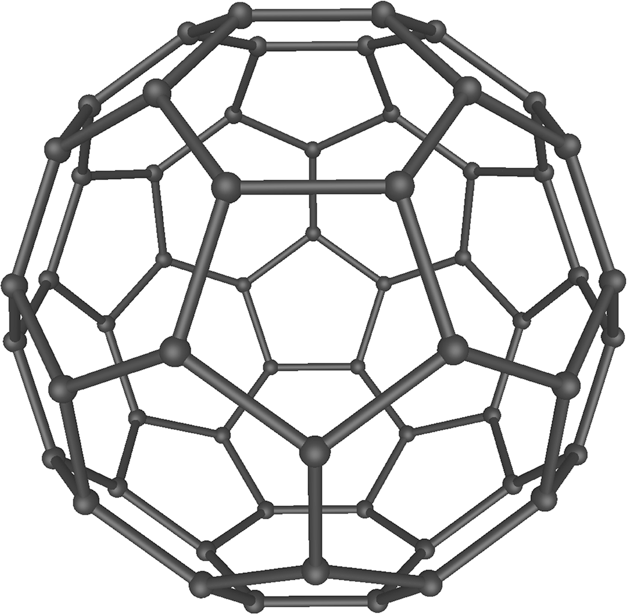
\includegraphics[scale = .2]{./Figures/C60a.png}
\caption{The structure of the $C_{60}$ molecule.}
\end{center}
\end{figure}


To access information in a vector or matrix you put the index you wish to access inside parentheses after the variable name. This works for both variable assignment and retrieval.

\begin{lstlisting}[style=matlab]
>> E(2,2)
ans =
     5
>> b(2)
ans =
     2
>> E(2,2) = 3
E =
     1     4     1     1     1
     2     3     4     2     1
     3     6     9     3     1  
\end{lstlisting}

The colon operator is used to retrieve an entire row or column from a matrix.  For example, enter the following to get the second column of a matrix:

\begin{lstlisting}[style=matlab]
>> E(:,2)
ans =
     4
     3
     6
\end{lstlisting}

We similarly retrieve the first row:

\begin{lstlisting}[style=matlab]
>> E(1,:)
ans =
     1     4     1     1     1
\end{lstlisting}

It is also possible to retrieve multiple columns or rows at once. For example, we retrieve the first and third columns of a matrix by entering:
\begin{lstlisting}[style=matlab]
>> E(:,[1 3])
ans =
     1     1
     2     4
     3     9
\end{lstlisting}

We list the entries of a matrix as a vector using the colon operator in the following way:

\begin{lstlisting}[style=matlab]
>> D(:)
ans =
     1
     2
     3
     4
     5
     6
\end{lstlisting}

Essentially, the colon operator tells MATLAB to return all valid entries in that dimension.

There is also a special keyword \li{end} that simply goes to the end of a matrix. The following line tells MATLAB to retrieve the entries in the second row, from the second column to the end:

\begin{lstlisting}[style=matlab]
>> E(2,2:end)
ans =
     3     4     2     1
\end{lstlisting}

Deleting a row or column can be done by assigning an empty matrix ([ ]) to it. For example:

\begin{lstlisting}[style=matlab]
>> E(:,2) = []
E =
     1     1     1     1
     2     4     2     1
     3     9     3     1
\end{lstlisting}
 
\begin{problem}
Try to assign a vector of incorrect size to a piece of a matrix. What happens? Also, try to concatenate two matrices that don't have matching dimensions. What error message do you get? It is important to learn how to read error messages for troubleshooting purposes.
\end{problem}

Basic matrix operations use the characters \li{+}, \li{-} and \li{*}. The transpose (or more precisely the adjoint) can be created by using an \li{'}. Also the \li{^} operator can be used to raise square matrices to a specific power.
\begin{lstlisting}[style=matlab]
>> b+c
ans =
     5
     7
     9
>> b-c
ans =
    -3
    -3
    -3
>> E*[1:4]'
ans =
    10
    20
    34
\end{lstlisting}

Operators can also act element-wise on a matrix by using a period. Experiment with the following:

\begin{lstlisting}[style=matlab]
>> b.*c
ans =
     4
    10
    18
>> b.^c
ans =
     1
    32
   729
>> b./c
ans =
    0.2500
    0.4000
    0.5000
\end{lstlisting}

The majority of elementary functions, such as \li{sin}, \li{cos} and \li{exp} act element-wise on matrices. For example:
\begin{lstlisting}[style=matlab]
>> sin([0:4]*pi/4)
ans =
         0    0.7071    1.0000    0.7071    0.0000    
\end{lstlisting}

There are a variety of functions that let us summarize information about a given matrix. For example, the \li{sum} function returns the sum of each column of a matrix:
\begin{lstlisting}[style=matlab]
>> sum(E)
ans =
     6    14     6     3
\end{lstlisting}

We can also specify the dimension that we want to sum across in our function call. For example, if instead we want to sum across rows we can write:

\begin{lstlisting}[style=matlab]
>> sum(E,2)
ans =
     4
     9
    16
\end{lstlisting}

Some other functions that summarize information about the entries of a matrix are contained in the Table \ref{tbl:summarizefuncs}. Note that each of these functions reduces the size of the matrix (which makes sense, since they are summarizing functions). These functions work across columns by default, although most of them allow you to specify a dimension to work across.

\begin{table}[h!]
\begin{center}
	\begin{tabular}{|c|c|}

    \hline

    Function & Usage \\

    \hline

    \li{max} & Returns maximum entries\\

    \li{min} & Returns mimimum entries\\

    \li{mean} & Returns the mean\\

    \li{median} & Returns the median\\

    \li{std} & Returns the standard deviation\\

    \li{diff} & Returns the differences between entries\\
    
    \li{prod} & Returns the product of entries\\
    
    \li{any} & Returns 1 if there are non-zero entries, zero otherwise\\
    
    \li{all} & Returns 1 if all entries are non-zero, zero otherwise\\

    \li{find} & Returns indices of non-zero entries\\

    \li{norm} & Returns the norm \\ 

    \hline

    \end{tabular}
\end{center}
\caption{Various summarizing functions}
\label{tbl:summarizefuncs}
\end{table}

These functions can be incredibly useful. For example, suppose that we want to estimate the derivative of $sin(x^2)$. A simple approximation for a derivative is
\[
f'(x) \approx \frac{f(x+h) - f(x)}{h}
\]

Presumably this approximation is good when $h$ is small. We use the \li{diff} function to perform this approximation using the following code:

\begin{lstlisting}[style=matlab]
>> h = .001;
>> x = 0:h:pi;
>> approx = diff(sin(x.^2))/h;
\end{lstlisting}

%More awkward wording.  Edit.
Here we evaluate the function $\sin{x}$ at several thousand points between $0$ and $\pi$.  Then, using the derivative estimation formula above, we calculate an approximation of the derivative at each point.  These results are stored in vector \li{approx}.  The analytic solution is:
%What we have done here is evaluate our function at a variety of points close together. We then use the difference of these points to calculate an approximation of the derivative. We have stored these values in the vector {\tt approx}. The actual derivative of this function, calculated by hand is:
\[
f'(x) = 2x cos(x^2)
\]
We write this function (evaluated at the same set of points) as:
\begin{lstlisting}[style=matlab]
>> actual = 2*cos(x.^2).*x;
\end{lstlisting}

%Wording
\begin{problem}
Plot the approximated derivative and the actual derivative on two different plots (the command \li{figure} opens a new plot window, which may be helpful). They should look almost identical. Now use the \li{max} command to find the maximum difference between the estimated derivative and the actual derivative (the dimensions will not match exactly (why?);  fix this by adding or removing an entry from one of the vectors).
\end{problem}

\begin{problem}
The command \li{rand(m,n)} returns a matrix where the entries are ``randomly'' drawn from a uniform distribution between zero and one. Create a vector with ten thousand entries using this command. The theoretical values for the mean($\mu$) and standard deviation($\sigma$) of a uniformly distributed random variable between $a$ and $b$ are
\begin{align*}
\mu &= \frac{a+b}{2} \\
\sigma &= \frac{b-a}{\sqrt{12}}
\end{align*}
These values are calculated using moment-generating functions. Use the functions \li{mean} and \li{std} on the vector you created earlier. How do these compare to the theoretical values?
\end{problem}

The canonical problem in linear algebra is solving the equation $Ax = b$ for x, where $A$ is an $n \times n$ matrix and $b$ is a  $1 \times n$ vector. In linear algebra you probably learned to solve this equation by calculating the matrix inverse. MATLAB calculates the inverse of a matrix using the command \li{inv}. For example, we create a random system $Ax =b$ and solve it using the \li{inv} function (you may check the caclucations by hand):

%Excellent demonstration but needs a bit of work
\begin{lstlisting}[style=matlab]
>> A = [1 5 2; 3 5 1; 4 7 2]
A =
   1   5   2
   3   5   1
   4   7   2
>> b = [1; 3; 11/3]
b =
   1.0000
   3.0000
   3.6667
>> sol = inv(A)*b
sol =
   0.66667
   0.33333
  -0.66667
\end{lstlisting}

Recall that a norm is a measurement on the size of a vector.  For example, the Euclidean norm measures the straight line distance from the origin to the ``end'' of a vector.

\[
\norm{x} = \sqrt{x_1^2 + ... + x_n^2}
\]

If the norm of the difference of two vectors is close to zero, then they are good approximations of each other.  The \li{norm} function calculates the euclidean norm of an input vector, and thus we use it to verify that our approximation of the derivative is close to the actual derivative:
% We then verify that we have solved the system by comparing {\tt A*sol} and {\tt b} using the {\tt norm} function:

\begin{lstlisting}[style=matlab]
>> norm(b-A*sol)
ans =  
   2.6273e-15
\end{lstlisting}

In addition to the \li{inv} function, MATLAB has an optimized, more general way to solve linear systems. This method is accessed using the backslash operator. We use this operator, and compare it to the solution we found using \li{inv} as follows:

\begin{lstlisting}[style=matlab]
>> sol2 = A\b
sol2 =
   0.66667
   0.33333
  -0.66667
>> norm(sol2-sol)
ans =
   3.3307e-16
\end{lstlisting}

We mentioned that the backslash operator is more efficient than using the function \li{inv}, meaning it returns a result faster. Create the following script to compare the efficiency of each method:

\lstinputlisting[style=matlab, style=fromfile]{./Source/Algorithms/solve_sys.m}

The \li{tic} and \li{toc} commands act as a stopwatch, allowing us to record execution time of various operations.

Now run the script. You should notice a significant difference in execution time (you may need to scale $n$ appropriately). This is because directly calculating a matrix inverse is costly, and MATLAB has optimized procedures for solving linear systems without calculating the inverse. Specifically, MATLAB uses the the LU factorization and backwards substitution to solve the linear system without any matrix inversions.

The backslash operator can also be used to solve several systems at once. For example:

\begin{lstlisting}[style=matlab]
>> A\[b c]
ans =
   -4.4458    6.0150
    7.9111   -1.3294
   -6.5331    5.8585
\end{lstlisting}

%Explain scripts
You might now be asking why we would want to do this. We can answer this by investigating the time it takes to solve two systems. Open a new script file and write the following:

\begin{lstlisting}[style=matlab]
n = 3000;
A = rand(n);
b = rand(n,1);
c = rand(n,1);

tic;
A\b;
A\c;
toc

tic;
A\[b c];
toc
\end{lstlisting}

This script creates a random $3000 \times 3000$ matrix, and two random $3000 \times 1$ vectors (you can experiment with different sizes of matrices and vectors). It then solves the two systems of equations twice, once using two backslash commands and the other using only one. Remember that the semi-colons suppress the output in the script.

Now execute this script. You should notice that the first method takes about twice as long as the second method. This is because the backslash method uses the LU decomposition, and in the second method it only has to execute this factorization once. This highlights the importance of understanding the algorithms that MATLAB uses: we can solve problems much faster if we understand what MATLAB is doing.

A number of other important operators that you will need are found in Table \ref{tbl:matrixops}.

\begin{table}[h!]
\begin{center}

    \begin{tabular}{|c|c|}

    \hline

    Function or Operator & Usage \\

    \hline

    \li{inv} & Matrix inverse\\

    \li{rank} & Rank\\

    \li{norm} & Norm (defaults to 2-norm)\\

    \li{expm} & Matrix exponential\\

    \li{det} & Determinant\\

    \li{eig} & Eigenvalue decomposition\\
    
    \li{svd} & Singular value decomposition\\
    
    \li{lu} & LU decomposition\\
    
    \li{qr} & QR factorization\\
    
    \li{chol} & Cholesky factorization\\

    \hline

    \end{tabular}
	\caption{Useful matrix operations}
\label{tbl:matrixops}
\end{center} 
\end{table}

%Explain better
\begin{problem}
The backslash operator can be also used to solve overdetermined systems. This is sometimes called the least squares method. The formula is $(A^TA)^{-1}A^T*b$. Create a script verify numerically that the backslash operator and the least squares formula yield the same result. Hint: Use the \li{norm} function to verify equality, as we did with \li{inv} and backslash.
\end{problem}
